\subsection{Čvorovi deklaracija}
\label{subsec:MyASTDeclarationNodes}

Kao što je opisano u odeljku \ref{sec:Paradigms}, u striktno tipiziranim proceduralnim jezicima promenljive i funkcije koje se koriste se moraju deklarisati pre trenutka njihovog korišćenja. Prateći kvalifikatori (statičnost, konstantnost itd.) i modifikatori pristupa (javni, privatni itd.) će se u nastavku nazivati \emph{specifikatori deklaracije} (engl. \emph{declaration specifiers}). Nakon specifikatora deklaracije dolazi konkretan \emph{deklarator}, koji ima specifičan oblik u zavisnosti od toga šta se deklariše. Oba imena su uzeta po uzoru na imena pravila gramatike programskog jezika C. 

Veliki broj proceduralnih jezika dozvoljava deklarisanje više promenljivih odjednom koje dele iste specifikatore deklaracije. Stoga specifikatore neće pratiti jedan deklarator, nego \emph{lista deklaratora}. Takođe, deklaratori u listi ne moraju biti samo deklaratori promenljivih --- moguće je deklarisati i nizovnu promenljivu zajedno sa deklaracijama običnih promenljivih. Na slici \ref{fig:DeclarationParts} se može videti dekompozicija deklaracije promenljive i niza u različitim proceduralnim programskim jezicima a na slici \ref{fig:DeclarationNodes} uočena hijerarhija sa podvrstama deklaratora.

\begin{figure}[h!]
\centering
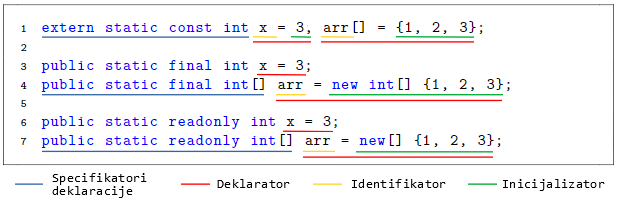
\includegraphics[scale=0.8]{images/declaration_decomposition.png}
\caption{Delovi deklaracije promenljive i niza prikazani na isečcima koda pisanog u programskim jezicima C, Java i C\#.}
\label{fig:DeclarationParts}
\end{figure}

\begin{figure}[h!]
\centering
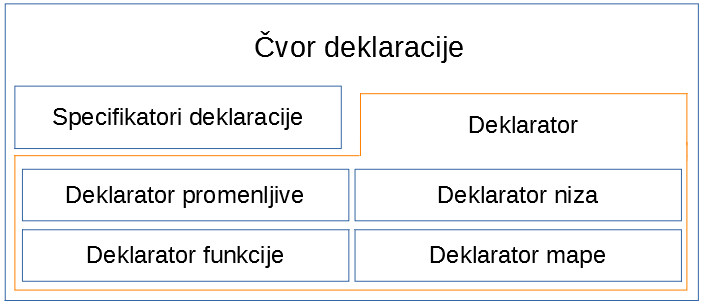
\includegraphics[scale=0.5]{images/declaration_nodes.png}
\caption{Prikaz vrsti AST čvorova deklaracije.}
\label{fig:DeclarationNodes}
\end{figure}

Kao što je prikazano na slici \ref{fig:DeclarationParts}, specifikatori deklaracije pokrivaju kvalifikatore, specifikatore pristupa i ime tipa. Pošto se pravi zajednička apstrakcija, potrebno je uočiti ekvivalenetne ključne reči u različitim programskim jezicima --- u primeru sa slike to su \texttt{const}, \texttt{final} i \texttt{readonly}. Imena tipova u programskim jezicima Java i C\# uzeta su po uzoru na programski jezik C, tako da tu ne vidimo razlike. U opštem slučaju, moguće je definisati mapiranje imena tipa u apstraktni tip. Ukoliko, na primer, posmatramo tipove koji predstavljaju realne brojeve, osim tipova \texttt{float} i \texttt{double}, postoji i tip \texttt{decimal}\footnote{Tip \texttt{decimal} predstavlja 128-bitni realan broj sa povećanom veličinom mantise a smanjenom veličinom eksponenta u odnosu na tip \texttt{double}. Koristi se pri numeričkm izračunavanjima gde preciznost primitivnih tipova realnih brojeva nije dovoljna.} prisutan u programskom jeziku C\#. Sva tri ova tipa mogu da se posmatraju na istom nivou apstrakcije kao tip realnih brojeva. Za korisnički definisane tipove isto ne može da se primeni.

Deklaratori za proceduralne jezike mogu biti deklaratori promenljive, niza ili funkcije i od toga zavisi njihov sastav. Svi deklaratori moraju sadržati informaciju o idenfitikatoru. Ukoliko je reč o deklaratoru niza, dodatno se očekuje i oznaka za niz (obično par srednjih zagrada --- \texttt{[]}) i opcioni izraz koji predstavlja dimenziju niza, obično unutar oznake niza. Ukoliko je reč o deklaratoru funkcije, pored identifikatora se očekuje i lista parametara funkcije obično navedena unutar para običnih zagrada. Lista parametara funkcije se može posmatrati rekurzivno --- svaki parametar se može posmatrati kao varijanta deklaracije --- sadrži specifikatore deklaracije (koji uključuju i tip) i deklarator, s tim što u ovom slučaju nije dozvoljeno da taj deklarator bude deklarator funkcije (pošto funkcije nisu građani prvog reda u imperativnoj paradigmi). 

Deklaratori promenljive i niza mogu dodatno sadržati i \emph{inicijalizator}. Inicijalizator možemo posmatrati kao opcioni izraz u slučaju deklaratora promenljive. U slučaju deklaratora niza, inicijalizator može biti lista izraza. Deklaratori funkcije ne mogu imati inicijalizatore.

U skript jezicima su uobičajeno podržane strukture podataka kao što su skupovi i mape. Stoga, kako bi se i mape mogle predstaviti apstraktno, dodat je tip deklaratora koji predstavlja deklarator mape. Mapa se sastoji od skupa ključeva pri čemu je svakom ključu dodeljena vrednost ne nužno istog tipa kao što je tip ključa. Mape postoje i u proceduralnim jezicima, ali ključna razlika je ta što tipovi u skript jezicima nisu striktni --- ključevi međusobno, ali i vrednosti mogu biti različitog tipa. Vredi naglasiti da se mape mogu porediti sa objektima određenih klasa --- svaki objekat se može serijalizovati u mapu gde su ključevi imena javnih atributa klase a vrednosti su vrednosti javnih atributa objekta koji se serijalizuje. Neki jezici (kao što je Python), imaju funkcije koje od objekta vraćaju baš ovakvu mapu. Ova ideja se dalje može proširiti kako bi se serijalizovale i metode klase, označila statička i privatna polja kao i sačuvale informacije o definisanim konstruktorima. Zatim je moguće porediti mape definisane u skript jezicima sa objektima iz proceduralnih jezika.

Na slici \ref{fig:MyASTExampleCDeclaration} se mogu videti kreirani AST za nekoliko deklaracija pisanih u programskom jeziku C a na slici \ref{fig:MyASTExampleLuaDeclaration} se može isto videti demonstracija \emph{automatske deklaracije} promenljivih za skript programski jezik Lua. Naime, pre prvog pojavljivanja identifikatora veštački će biti deklarisan taj identifikator, kako bi razlika između apstrakcija dobijenih iz proceduralnih i skript jezika bila što manja. U ovom slučaju će se deklaracija i dodela spojiti u deklaraciju sa inicijalizatorom.

\begin{figure}[h!]
\begin{lstlisting}
extern int y = 3;
static int arr[5] = { 1 };
\end{lstlisting}
\centering
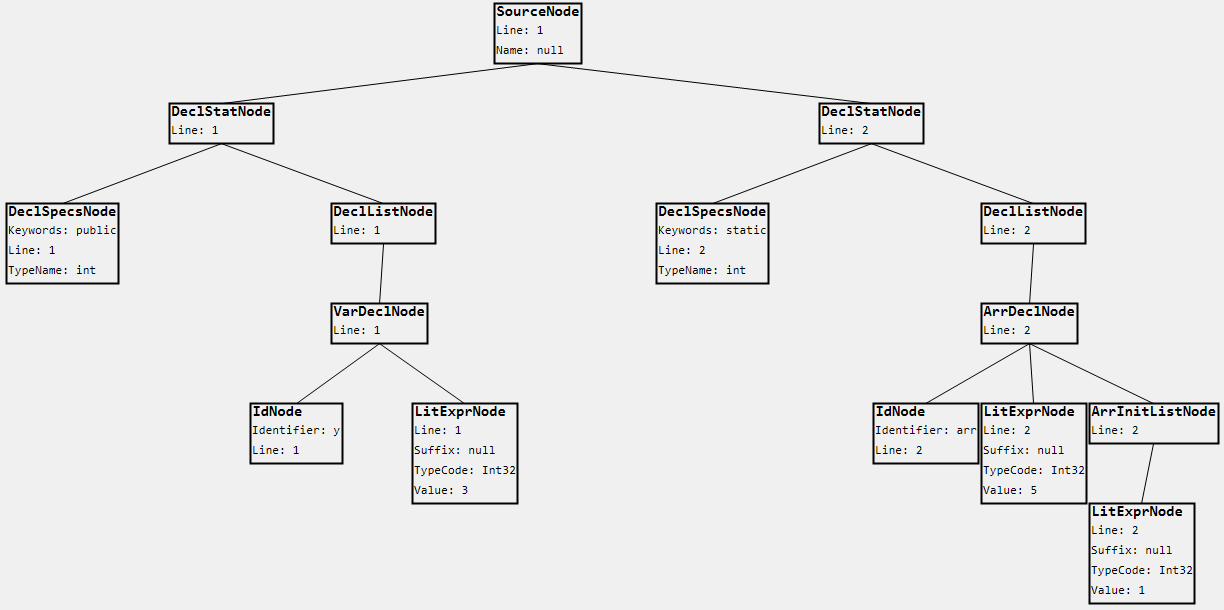
\includegraphics[scale=0.48]{images/c_ast_decl2.png}
\caption{Primer deklaracije promenljive i niza u programskom jeziku C i odgovarajući AST.}
\label{fig:MyASTExampleCDeclaration}
\end{figure}

\begin{figure}[h!]
\begin{lstlisting}
arr = { 1, 2 }
dict = { a = 1 }
\end{lstlisting}
\centering
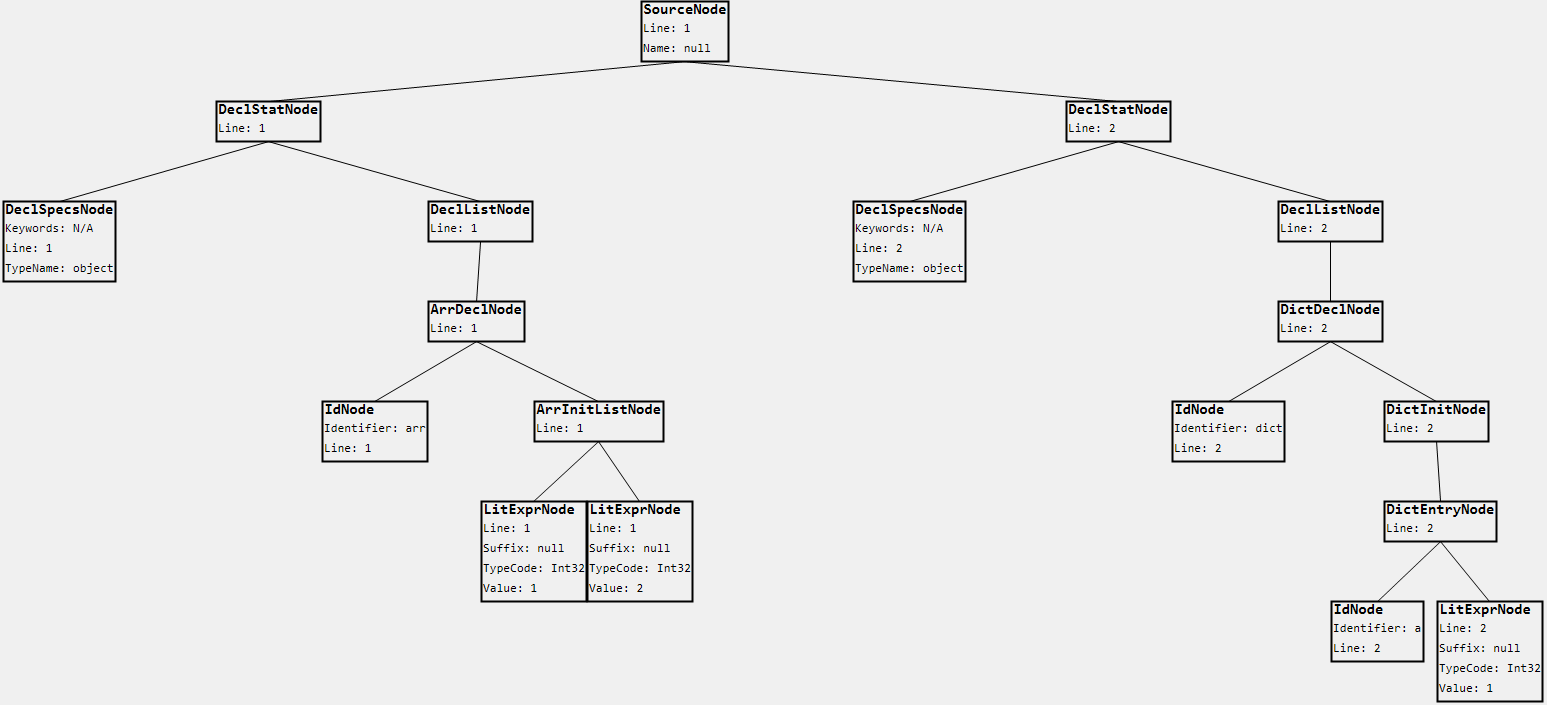
\includegraphics[scale=0.4]{images/lua_ast_decl.png}
\caption{Primer deklaracije promenljive i niza u programskom jeziku Lua i odgovarajući AST.}
\label{fig:MyASTExampleLuaDeclaration}
\end{figure}

